%%%%%%%%%%%%%%%%%%%%%%%%%%%%%%%%%%%%%%%%%
% Tutorial
% LaTeX Template
% Version 1.0 (09/27/17)
%
% Author:
% Ben Roose (ben.roose@wichita.edu)
%
% Original template author:
% Adam Glesser (adamglesser@gmail.com)
% www.LaTeXTemplates.com
%
% License:
% CC BY-NC-SA 3.0 (http://creativecommons.org/licenses/by-nc-sa/3.0/)
%
%%%%%%%%%%%%%%%%%%%%%%%%%%%%%%%%%%%%%%%%%

\documentclass[12pt]{article}

\usepackage{graphicx} % Allow import of images
\usepackage{subcaption} % Required for side-by-side sub figures
\graphicspath{ {images/} } % Relative path to images directory
\usepackage[margin=1in]{geometry} % Required to make the margins smaller to fit more content on each page
\usepackage[linkcolor=blue]{hyperref} % Required to create hyperlinks to questions from elsewhere in the document
\hypersetup{pdfborder={0 0 0}, colorlinks=true, urlcolor=blue} % Specify a color for hyperlinks
\usepackage{todonotes} % Required for the boxes that questions appear in
\usepackage{tocloft} % Required to give customize the table of contents to display questions
\usepackage{microtype} % Slightly tweak font spacing for aesthetics
\usepackage{palatino} % Use the Palatino font

\setlength\parindent{0pt} % Removes all indentation from paragraphs

% Create and define the list of questions
\newlistof{questions}{faq}{\large FAQ for SSH access into cslab Linux environment}
% This creates a new table of contents-like environment that will output a file with extension .faq
\setlength\cftbeforefaqtitleskip{3em} % Adjusts the vertical space between the title and subtitle
\setlength\cftafterfaqtitleskip{1em} % Adjusts the vertical space between the subtitle and the first question
\setlength\cftparskip{.3em} % Adjusts the vertical space between questions in the list of questions

% Create the command used for questions
\newcommand{\question}[1] % This is what you will use to create a new question
{
\refstepcounter{questions} % Increases the questions counter, this can be referenced anywhere with \thequestions
%\hfill
\goodbreak
\par\noindent % Creates a new unindented paragraph
\phantomsection % Needed for hyperref compatibility with the \addcontensline command
\addcontentsline{faq}{questions}{#1} % Adds the question to the list of questions
\todo[inline, color=green!40]{\textbf{#1}} % Uses the todonotes package to create a fancy box to put the question
%\vspace{0.5em} % White space after the question before the start of the answer
}

% Uncomment the line below to get rid of the trailing dots in the table of contents
%\renewcommand{\cftdot}{}

% Uncomment the two lines below to get rid of the numbers in the table of contents
%\let\Contentsline\contentsline
%\renewcommand\contentsline[3]{\Contentsline{#1}{#2}{}}

\begin{document}

%----------------------------------------------------------------------------------------
%	TITLE AND LIST OF QUESTIONS
%----------------------------------------------------------------------------------------

\begin{center}
\Huge{\bf \emph{EECS Tutorial: cslab Linux Environment SSH Access}} % Main title
\end{center}

\listofquestions % This prints the subtitle and a list of all of your questions
\bigskip % Create a gap between list and first question

\newpage % Comment this if you would like your questions and answers to start immediately after table of questions

%----------------------------------------------------------------------------------------
%	QUESTIONS AND ANSWERS
%----------------------------------------------------------------------------------------
\begin{flushleft}

\question{General Information regarding accessing cslab Linux environment using SSH}\label{ssh_client_linux}
\begin{itemize}
  \item \textbf{Please only connect into the cslab environment with an SSH client if you have previous experience in using SSH and the Linux command-line. If you are new to Linux, please use the cslab \textit{Guacamole} web-browser interface.}
  \item SSH uses network port 22. If you are accessing cslab via SSH on WSU campus, ensure you are connected wirelessly to ``WSU Secure'' or using an Ethernet connected computer. ``WSU Guest'' wireless prohibits port 22 connections and your SSH session will fail to connect.
  \item You can only access cslab using SSH public key authentication. You cannot access cslab over SSH using your myWSU password.
  \item The cslab-nodes are located inside a virtual private network. These internal nodes are only SSH accessible via the \texttt{cslab-bastion.cs.wichita.edu} jumphost. Any external connection into the cslab environment must proxy connect through the \texttt{cslab-bastion}.
  \item \texttt{cslab-bastion.cs.wichita.edu} and \texttt{cslab-sftp.cs.wichita.edu} can be used as SCP or SFTP file-server hosts with SSH clients, such as \textit{OpenSSH}, or graphical SFTP clients, such as \textit{Filezilla}.
  \item This tutorial will help you configure your SSH client to make a proxy connection into cslab via \texttt{cslab-bastion} and to set up SSH public key authentication.
  \item \textbf{ONLY USE THE CSLAB-BASTION AS A PROXY/JUMPHOST INTO THE CSLAB-NODES OR AS AN SCP/SFTP SERVER. DO NOT DIRECTLY SSH INTO THE CSLAB-BASTION FOR OTHER TASKS!}
\end{itemize}

%------------------------------------------------
\newpage
\question{How do I access cslab Linux environment via \textit{PuTTY} on Microsoft Windows?}\label{ssh_client_windows}
  
\subsection*{Configuring the \textit{PuTTY} SSH client for cslab access:}
\begin{enumerate}
%% \item You can download pre-configured \textit{PuTTY} session and host key configurations for importing into your Windows registry from this link.

  \item Download the full \textit{PuTTY} package from \href{https://www.chiark.greenend.org.uk/~sgtatham/putty/latest.html}{Simon Tatham's official download page} and install all \textit{PuTTY} utilities on your local Windows computer. You cannot connect to cslab with just the \textit{PuTTY} client.
  \item Run the \textit{PuTTY Key Generator}, which is listed in your start menu as \textit{PuTTYgen}.
  \item In the \textit{PuTTY Key Generator} window, generate a new RSA key with 4096 bits. You may need to change the settings at bottom of window before clicking \textbf{Generate}.
  \item Follow the prompts to create randomness and generate your RSA key.
  \item Once your key has been generated, change the following fields:
    \begin{itemize}
    \item Key comment: \texttt{your\_mywsu\_id@your\_local\_computer\_name}
    \item Key passphrase: \texttt{choose\_passphrase\_you\_will\_remember}
    \item Confirm passphrase: \texttt{same\_passphrase\_as\_above}
    \end{itemize}
    \textbf{It is highly recommended to use a passphrase for your RSA key to keep your Linux user account secure.}
  \item Select all the text displayed within the box titled \textit{Public key for pasting into OpenSSH authorized\_keys file}, starting with \texttt{ssh-rsa} and ending with name of your computer.
  \item Copy the selected text either by right-clicking within the same box and selecting [copy] or by pressing the key combination \textbf{Ctrl+C}.
  \item Open a web-browser application and follow the \textit{eecs\_tutorial\_cslab\_web\_access} document to access \href{https://cslab-gateway.cs.wichita.edu/}{cslab-gateway.cs.wichita.edu}
  \item Once logged into \textit{guacamole}, open a [cslab\_SSH\_CLI\_terminal] connection.
  \item Within the cslab SSH terminal session in your browser, open the \textit{Guacamole} menu sidebar by pressing the key combination \textbf{Ctrl+Alt+Shift}.
  \item Paste the copied text to the remote \textit{Guacamole} \textbf{Clipboard} field using your preferred method, i.e. \textbf{Ctrl+V}.
  \item Close the \textit{Guacamole} menu sidebar by pressing the key combination \textbf{Ctrl+Alt+Shift}.
  \item Within the cslab SSH terminal session, open your \texttt{authorized\_keys} file by typing \break
  \texttt{nano $\sim$/.ssh/authorized\_keys}
  \item Paste your locally copied SSH public key into the terminal session by right-clicking on the browser window with your mouse or by pressing the key combination \textbf{Ctrl+Shift+V}.
  \item Ensure you have a blank line at end of the text file by pressing \textbf{Enter} if required.
  \item Quit \textit{nano} by pressing \textbf{CTRL+X} and follow the prompts at the bottom of the screen to ensure you save the \texttt{authorized\_keys} file.
  \item Ensure correct permissions are set on the \texttt{authorized\_keys} file by typing \break
  \texttt{chmod 600 $\sim$/.ssh/authorized\_keys}
  \item NOTE: If you wish to set up more than one local computer with different SSH keys for accessing cslab, then you can append additional SSH public keys in your cslab user \texttt{authorized\_keys} file. Make sure to remove no longer used SSH public keys from this file.
  \item Once you are done with the above steps, make sure to properly disconnect and log out of the cslab \textit{guacamole} web-interface.
  \item Back in the \textit{PuTTY Key Generator} window, click \textbf{Save private key}.
  \item In the \textit{Save private key} window, browse to a local directory where you wish to securely store your new SSH key and in the \textbf{File name} field enter the name \texttt{cslab\_rsa}. Clicking on \textbf{Save} will store your SSH key to your local computer as the \texttt{cslab\_rsa.ppk} \textit{PuTTY} key file. \textbf{Keep this file safe and private!}
  \item OPTIONAL: If you wish to also store your SSH public key as a simple text file for future reference, then click \textbf{Save public key}, browse to the same directory, and in the \textbf{File name} field enter the name \texttt{cslab\_rsa\_public\_key.txt}
  \item Once you are done with the above steps, exit/close the \textit{PuTTY Key Generator} program.
  \item Download the \texttt{cslab\_putty\_ssh\_client\_full\_configuration} registry file from \href{https://github.com/benroose/tutorials/tree/master/cslab_ssh_client_config_files}{Ben Roose's GitHub tutorials repository}.
  \item Open this downloaded file from within your web-browser or by double-clicking on the file in your file explorer, and click \textbf{Yes} when asked if you wish to add this new information to your Windows registry. You will not be able to continue configuration of PuTTY until this file has been added into your Windows registry.
  \item Run the \textit{PuTTY} program and you should now see two new \textbf{Saved Sessions} entries in your \textit{PuTTY} Configuration Window listed as \textit{cslab access} and \textit{cslab last node accessed}.
  \item Click on \textit{cslab access} and click on \textbf{Load}. DO NOT click \textbf{Open}.
  \item Click on the \textit{Connection--Data} Category tab on the left of the window and enter your myWSU ID in the \textbf{Auto-login username} field.
  \item Click on the \textit{Connection--Proxy} Category tab on the left of the window and enter your myWSU ID in the \textbf{Username} field.
  \item Click on the \textit{Session} Category tab on the left of the window and click on \textbf{Save}. DO NOT click \textbf{Open}.
  \item Perform the last 4 steps again for the \textit{cslab last node accessed} entry.
  \item Once you are done with the above steps, exit/close the \textit{PuTTY} program.
  \item Congratulations! You have now configured your local Windows computer to directly access cslab via \textit{PuTTY}. However, you will need to first add your new SSH key to the \textit{Pageant (PuTTY Authentication agent)} prior to logging into cslab. Running \textit{Pageant} and adding your SSH key will be explained in the next section!
\end{enumerate}

\begin{figure}[bh!]
\centering
\begin{subfigure}{.5\textwidth}
  \centering
  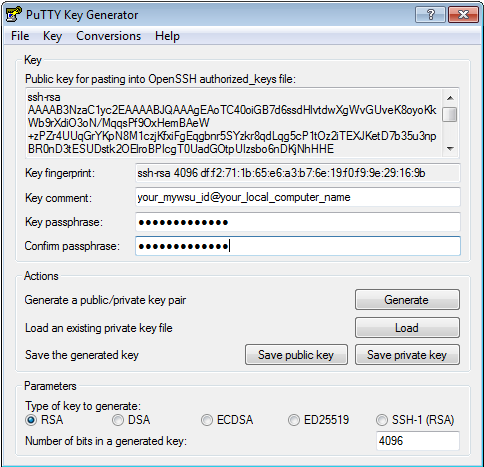
\includegraphics[width=.9\linewidth]{puttygen_key_gen_fields}
  %% \caption{A subfigure}
  \label{fig:sub1}
\end{subfigure}%
\begin{subfigure}{.5\textwidth}
  \centering
  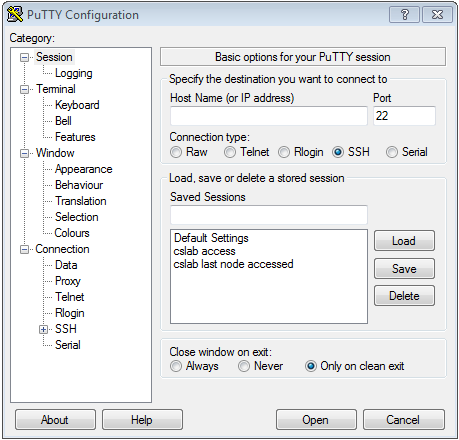
\includegraphics[width=.9\linewidth]{putty_cslab_session_tab}
  %% \caption{A subfigure}
  \label{fig:sub2}
\end{subfigure}
\begin{subfigure}{.5\textwidth}
  \centering
  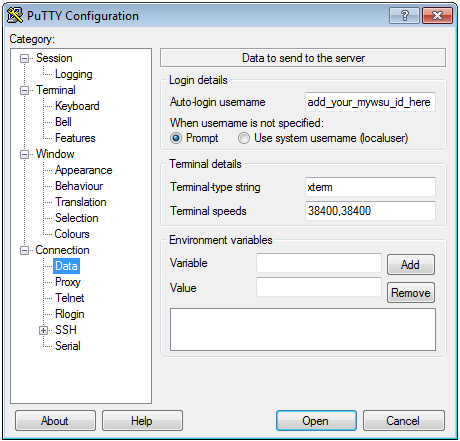
\includegraphics[width=.9\linewidth]{putty_cslab_data_tab}
  %% \caption{A subfigure}
  \label{fig:sub3}
\end{subfigure}%
\begin{subfigure}{.5\textwidth}
  \centering
  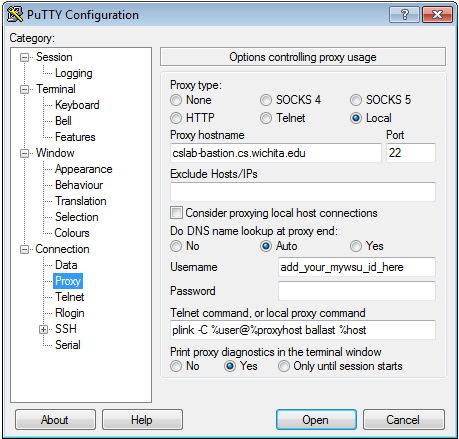
\includegraphics[width=.9\linewidth]{putty_cslab_proxy_tab}
  %% \caption{A subfigure}
  \label{fig:sub4}
\end{subfigure}%
\caption{\textit{PuTTY} screenshots for cslab configuration}
\label{fig:putty_config}
\end{figure}

\newpage
\subsection*{Logging into cslab using the \textit{PuTTY Pageant} client:}
\begin{enumerate}
  \item Run the \textit{Pageant (PuTTY Authentication agent)}, listed in your start menu as \textit{Pageant}.
  \item On the far right of your Windows taskbar, you should see a new notification icon for the running \textit{Pageant} program.
  \item Right-click on the \textit{Pageant} notification icon and select the menu option \textbf{Add key}.
  \item In the \textit{Select private Key File} window, browse to the local directory with your stored \texttt{cslab\_rsa.ppk} file. Select the \texttt{cslab\_rsa} key file and click on \textbf{Open}.
  \item When prompted, enter the previously defined passphrase for your key.
  \item OPTIONAL: if you wish to see the SSH keys already added into \textit{Pageant}, right-click on the \textit{Pageant} notification icon and select the menu option \textbf{View keys}.
  \item Right-click on the \textit{Pageant} notification icon and, under the \textbf{Saved Sessions} sub-menu, select \textbf{cslab remote access}.
  \item If everything is correctly configured, a new \textit{PuTTY} terminal emulator window will open and automatically log you into an available cslab node!
  \item Each time you shutdown or reboot your computer, you will need to manually run \textit{Pageant} and then add your SSH key before you can connect to the cslab environment.
  \item OPTIONAL: You can have \textit{Pageant} run automatically at startup by copying the \textit{Pageant} Start menu shortcut file into your Windows \textbf{Startup} directory.
  \item OPTIONAL: To have your cslab SSH key automatically added into \textit{Pageant} when it runs, open the \textbf{Properties} box for the \textit{Pageant} Start menu shortcut (or the \textbf{Startup} shortcut). In the \textbf{Target} field enter the full filepath of your \texttt{cslab\_rsa.ppk} key file to the end of the \texttt{pageant.exe} line, i.e.
\end{enumerate}
  \begin{verbatim}
"C:\Program Files\PuTTY\pageant.exe" "C:\Users\localuser\cslab_rsa.ppk"
  \end{verbatim}

\begin{figure}[bh!]
  \centering
  %% \begin{subfigure}{.5\textwidth}
  \centering
  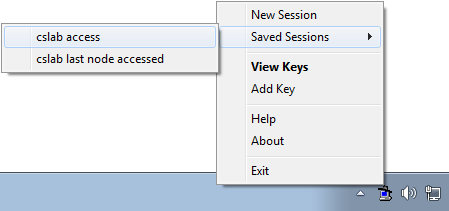
\includegraphics[width=.5\linewidth]{pageant_taskbar_menu}
\caption{\textit{Pageant} taskbar menu for cslab access}
  \label{fig:pageant}
%% \end{subfigure}%
\end{figure}

%------------------------------------------------
\newpage
\subsection*{Logging into your last used cslab-node-\# using the \textit{PuTTY} client:}
\begin{itemize}
  \item When connecting to the cslab Linux environment using an SSH client, the ballast load-balancer will redirect you to one of the available and least used cslab-nodes at time of connection. Since load-balancing is calculated by ballast on a one minute cycle, you may not be redirected to the same cslab-node each time you connect.

  \item \textbf{Use the \textit{cslab last node accessed} saved session to connect to the last used cslab-node only when you need access into a previously running SSH session. For normal use, the best option is to connect using the \textit{cslab access} saved session and let the ballast load-balancer automatically connect to an available node.}
\end{itemize}

\subsection*{Running graphical (GUI) applications using the \textit{PuTTY} client:}
\begin{enumerate}
  \item SSH allows for graphical applications to run on a local computer from the remote cslab Linux environment using X11 forwarding.
  \item You will need to install the Xming software before using X11 forwarding with \textit{PuTTY}. Download the \href{http://sourceforge.net/project/downloading.php?group_id=156984&filename=Xming-6-9-0-31-setup.exe}{Xming X Server for Windows} and install the software package.
  \item Run the \textit{PuTTY} program, click on \textbf{cslab access} in Saved Sessions, and click on \textbf{Load}.
  \item Click on the \textit{Connection--SSH--X11} Category tab on the left of the window.
  \item Turn on the \textbf{Enable X11 Forwarding} check box and ensure the \textbf{X display location} contains \texttt{localhost:0.0}. If you change the display location within \textit{Xming Launch} settings, then also change the \textbf{X display location} in \textit{PuTTY} to ensure consistency.
  \item Click on the \textit{Session} Category tab on the left of the window. Save this change as a different \textbf{Saved Session} by entering a new name for the session, such as \texttt{cslab with graphical access}, and click on \textbf{Save}.
  \item Once you are done with the above steps, exit/close the \textit{PuTTY} program.
  \item To use cslab with X11 forwarding run \textit{Xming} in the background first, then select your new \textbf{Saved Session} from the \textit{Pageant} notification menu.
  \item Once a connection into cslab has been established, you can type the name of a GUI application you wish to run, such as \texttt{geany}.
\end{enumerate} 

%% \begin{figure}[bh!]
%%   \centering
%%   %% \begin{subfigure}{.5\textwidth}
%%   \centering
%%   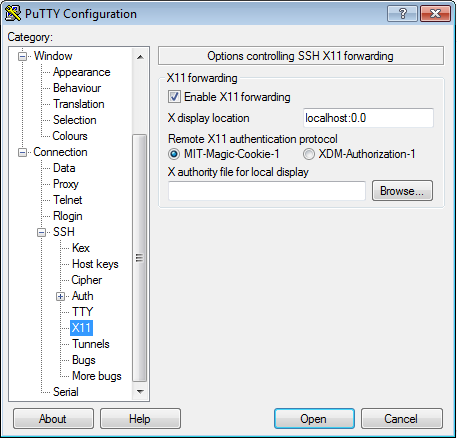
\includegraphics[width=.5\linewidth]{cslab_x11_tab}
%% %% \caption{\textit{PuTTY} Enable X11 Forwarding}
%%   \label{fig:x11_forwarding}
%% %% \end{subfigure}%
%% \end{figure}

%------------------------------------------------
\newpage
\question{Why is \textit{PuTTY} asking me to confirm the authenticity of cslab host?}\label{ssh_client_windows}

\begin{itemize}
  \item SSH host keys are essential to securing an SSH connection into a remote server. If you see an incorrect host key, then it may mean a cyber-attacker has attempted to compromise the remote server.
  \item The \texttt{cslab\_putty\_ssh\_client\_full\_configuration} file from \href{https://github.com/benroose/tutorials/tree/master/cslab_ssh_client_config_files}{Ben Roose's GitHub tutorials repository} will automatically add the cslab host keys into your Windows registry when you add this file during the initial configuration and set up of \textit{PuTTY}. However, if your configuration lost the host keys for any reason, then it may ask you to confirm the authenticity of cslab hosts when you try to open an SSH connection.
  \item You can also download the \texttt{cslab\_putty\_ssh\_client\_host\_keys\_only} file from \href{https://github.com/benroose/tutorials/tree/master/cslab_ssh_client_config_files}{Ben Roose's GitHub tutorials repository} and re-add the host keys into your Windows registry.
  \item Alternatively, you can manually add SSH host keys to your \textit{PuTTY} Session configurations. When adding new host keys you should always ensure the host key fingerprint is correct. cslab-bastion and cslab host key fingerprints must match one of the following SHA256 or MD5 hashes before you add or accept the host key:
\begin{verbatim}
ECDSA key fingerprint is
SHA256:X6dBKj4sqYYPWol6MXSQvGhpIQ6qBxh7mBQhnSw8n64
MD5:d8:ba:c6:1c:86:fa:7f:f6:92:4f:c1:02:30:ce:ab:99

ED25519 key fingerprint is
SHA256:zzozIV7cP1T9C77PLRaevzdzCu21k44lbjd8jaJKS8Q
MD5:6d:3d:8e:3a:db:f6:de:33:af:77:01:40:f3:71:1d:14

RSA key fingerprint is
SHA256:0CUyGZAYMdOd8vTOK3AtM2XTX3lMaGA2NP73rR7s6Ns
MD5:75:5a:16:53:1a:7c:c2:4b:99:66:2d:e3:1e:76:f9:c9

DSA key fingerprint is
SHA256:7zW122xr+aoBb5yiRI96nvdx8Ml07qLKHYwG2Wu6jIM
MD5:27:59:53:18:5a:67:71:f6:32:f1:e1:15:e9:e5:fe:b1
\end{verbatim}

\end{itemize}

%------------------------------------------------
\newpage
\question{How do I access cslab Linux environment via \textit{OpenSSH} on Linux or Mac?}\label{ssh_client_linux}

\subsection*{Configuring the \textit{OpenSSH} client for cslab access:}
\begin{enumerate}
  \item On your Linux or Mac desktop/laptop computer, copy the following host entry into your local user \texttt{$\sim$/.ssh/config} file:
\end{enumerate}

\begin{verbatim}
Host cslab cslab-last cslab.cs.wichita.edu cslab-last.cs.wichita.edu
  ProxyCommand ssh your_mywsu_id@cslab-bastion.cs.wichita.edu ballast %h
  User your_mywsu_id
  IdentityFile ~/.ssh/cslab_rsa
  HostKeyAlias cslab.cs.wichita.edu

Host cslab-sftp cslab-sftp.cs.wichita.edu
  HostName cslab-sftp.cs.wichita.edu
  User your_mywsu_id
  IdentityFile ~/.ssh/cslab_rsa
  HostKeyAlias cslab.cs.wichita.edu
\end{verbatim}
(Note: replace ``your\_mywsu\_id'' with your own 8 character ID number in both \texttt{ProxyCommand} and \texttt{User} lines.)

\begin{enumerate}
  \setcounter{enumi}{1}
  \item The above text is also available for download in the file \texttt{cslab\_openssh\_client\_config} from \href{https://github.com/benroose/tutorials/tree/master/cslab_ssh_client_config_files}{Ben Roose's GitHub tutorials repository}.
  \item Open a command-line terminal emulator window and generate a new SSH public/private key pair for your local user by typing \break
  \texttt{ssh-keygen -t rsa -b 4096 -f $\sim$/.ssh/cslab\_rsa}

  \item Follow the prompts in the command-line as your new SSH key is generated and enter a passphrase you will remember! \break
  \textbf{It is highly recommended to use a passphrase for your SSH key to keep your Linux user account secure.}
  
  \item Open the newly generated SSH public key by typing \break
  \texttt{less $\sim$/.ssh/cslab\_rsa.pub}
  \item Select all the text displayed within \textit{less}, starting with \texttt{ssh-rsa} and ending with hostname of your computer.
  \item Copy the selected text either by right-clicking on the terminal emulator window and selecting [copy] or by pressing the key combination \textbf{Ctrl+Shift+C}.
  \item Open a web-browser application and follow the \textit{eecs\_tutorial\_cslab\_web\_access} document to access \href{https://cslab-gateway.cs.wichita.edu/}{cslab-gateway.cs.wichita.edu}
  \item Once logged into \textit{guacamole}, open a [cslab\_SSH\_CLI\_terminal] connection.
  \item Within the cslab SSH terminal session in your browser, open the \textit{Guacamole} menu sidebar by pressing the key combination \textbf{Ctrl+Alt+Shift}.
  \item Paste the copied text to the remote \textit{Guacamole} \textbf{Clipboard} field using your preferred method, i.e. \textbf{Ctrl+V}.
  \item Close the \textit{Guacamole} menu sidebar by pressing the key combination \textbf{Ctrl+Alt+Shift}.
  \item Within the cslab SSH terminal session, open your \texttt{authorized\_keys} file by typing \break
  \texttt{nano $\sim$/.ssh/authorized\_keys}
  \item Paste your locally copied SSH public key into the terminal session by right-clicking on the browser window with your mouse or by pressing the key combination \textbf{Ctrl+Shift+V}.
  \item Ensure you have a blank line at end of the text file by pressing \textbf{Enter} if required.
  \item Quit \textit{nano} by pressing \textbf{CTRL+X} and follow the prompts at the bottom of the screen to ensure you save the \texttt{authorized\_keys} file.
  \item Ensure correct permissions are set on the \texttt{authorized\_keys} file by typing \break
  \texttt{chmod 600 $\sim$/.ssh/authorized\_keys}
  \item NOTE: If you wish to set up more than one local computer with different SSH keys for accessing cslab, then you can append additional SSH public keys in your cslab user \texttt{authorized\_keys} file. Make sure to remove no longer used SSH public keys from this file.
  \item Congratulations! You have now configured your local Linux or Mac computer to directly access cslab via \textit{OpenSSH}. Make sure to properly disconnect and log out of the cslab \textit{guacamole} web-interface once you are done with the above steps.
\end{enumerate}

\newpage
\subsection*{Logging into cslab using the \textit{OpenSSH} client:}
\begin{enumerate}
  \item Ensure you have first followed the directions in the previous section to configure your \textit{OpenSSH} client.
  \item In your local computer open a command-line terminal emulator window, such as \textit{lxterminal} or \textit{terminator}.
  \item Start the ssh-agent in the background by typing \texttt{eval "\$(ssh-agent -s)"}
  \item Add your cslab\_rsa private key to the ssh-agent by typing \texttt{ssh-add $\sim$/.ssh/cslab\_rsa}
  \item When prompted, enter your previously created passphrase to unlock your SSH private key.
  \item Connect to the cslab Linux environment by typing \texttt{ssh cslab}
  \item The first time you connect to the cslab environment using SSH, you will be asked to confirm the authenticity of each remote host, i.e.
\begin{verbatim}
The authenticity of host 'cslab.cs.wichita.edu' can't be established.
ECDSA key fingerprint is [SHA256 or MD5 hash value].
Are you sure you want to continue connecting (yes/no)?
\end{verbatim}

%\break
  \item Ensure the cslab-bastion and cslab host key fingerprints match one of the following SHA256 or MD5 hashes before typing \texttt{yes}:
\begin{verbatim}
ECDSA key fingerprint is
SHA256:X6dBKj4sqYYPWol6MXSQvGhpIQ6qBxh7mBQhnSw8n64
MD5:d8:ba:c6:1c:86:fa:7f:f6:92:4f:c1:02:30:ce:ab:99

ed25519 key fingerprint is
SHA256:zzozIV7cP1T9C77PLRaevzdzCu21k44lbjd8jaJKS8Q
MD5:6d:3d:8e:3a:db:f6:de:33:af:77:01:40:f3:71:1d:14

RSA key fingerprint is
SHA256:0CUyGZAYMdOd8vTOK3AtM2XTX3lMaGA2NP73rR7s6Ns
MD5:75:5a:16:53:1a:7c:c2:4b:99:66:2d:e3:1e:76:f9:c9

DSA key fingerprint is
SHA256:7zW122xr+aoBb5yiRI96nvdx8Ml07qLKHYwG2Wu6jIM
MD5:27:59:53:18:5a:67:71:f6:32:f1:e1:15:e9:e5:fe:b1
\end{verbatim}

  \item If the SSH connection completed successfully, then you will be presented with a standard shell prompt within a cslab node:\break
\texttt{your\_mywsu\_id@cslab-node-\#:$\sim$\$}
  \item NOTE: Mac OSX and many Linux distributions can run the ssh-agent and unlock SSH keys during user login using a \textit{keychain} program. Check online for specific details on how to store SSH keys in your distribution. If not, then there are many script functions that can be added to your local user \texttt{.bashrc} file for running the ssh-agent at login, such as \href{https://gist.github.com/tstellanova/76ee01c1599d9a9433cf}{tstellanova's start\_ssh\_agent.sh on GitHubGist}.
\end{enumerate}

\subsection*{Logging into your last used cslab-node-\# using the \textit{OpenSSH} client:}
\begin{itemize}
  \item When connecting to the cslab Linux environment using \texttt{ssh cslab}, the ballast load-balancer will redirect you to one of the available and least used cslab-nodes at time of connection. Since load-balancing is calculated by ballast on a one minute cycle, you may not be redirected to the same cslab-node each time you connect.

  \item \textbf{Only connect to the last used cslab-node if you need access into a previously running SSH session. For normal use, best option is always let the ballast load-balancer automatically connect to an available node.}
  \item To connect to the last node you previously accessed using SSH type \break
  \texttt{ssh cslab-last}
\end{itemize}

\subsection*{Running graphical (GUI) applications using the \textit{OpenSSH} client:}
\begin{itemize}
  \item SSH allows for graphical applications to run on a local computer from the remote cslab Linux environment using X11 forwarding.
  \item If you are using Mac OSX, then you may need to install the XQuartz software before using X11 forwarding. Download \href{https://www.xquartz.org}{XQuartz for Mac} and install the software package.
  \item To use X11 forwarding on a per session basis append the \texttt{-X} option flag to your SSH command: \break
  \texttt{ssh -X cslab}
\item To always use X11 forwarding for connections into cslab, instead of using the \texttt{-X} option flag, add the following line to the \texttt{Host cslab cslab-last} entry in your local user \texttt{ $\sim$/.ssh/config} file: \newline
  \texttt{ForwardX11 yes}
\end{itemize} 

%------------------------------------------------
%% \question{How do I copy files from/to the cslab Linux environment via an SSH client?}\label{scp_copying}

\subsection*{Copying files to/from cslab via SCP:}
\begin{itemize}
\item To copy a file from your local computer to your user home directory on cslab using Secure Copy (SCP), type \break
\texttt{scp local\_filename\_or\_path cslab-sftp:$\sim$}

\item To copy a file from your user home directory on cslab to a local directory on your local computer, type \break
\texttt{scp cslab-sftp:$\sim$/remote\_filename\_or\_path local\_directory}
\end{itemize}

%------------------------------------------------

\end{flushleft}
\end{document}
